% Created by tikzDevice version 0.12.3.1 on 2022-05-11 22:30:43
% !TEX encoding = UTF-8 Unicode
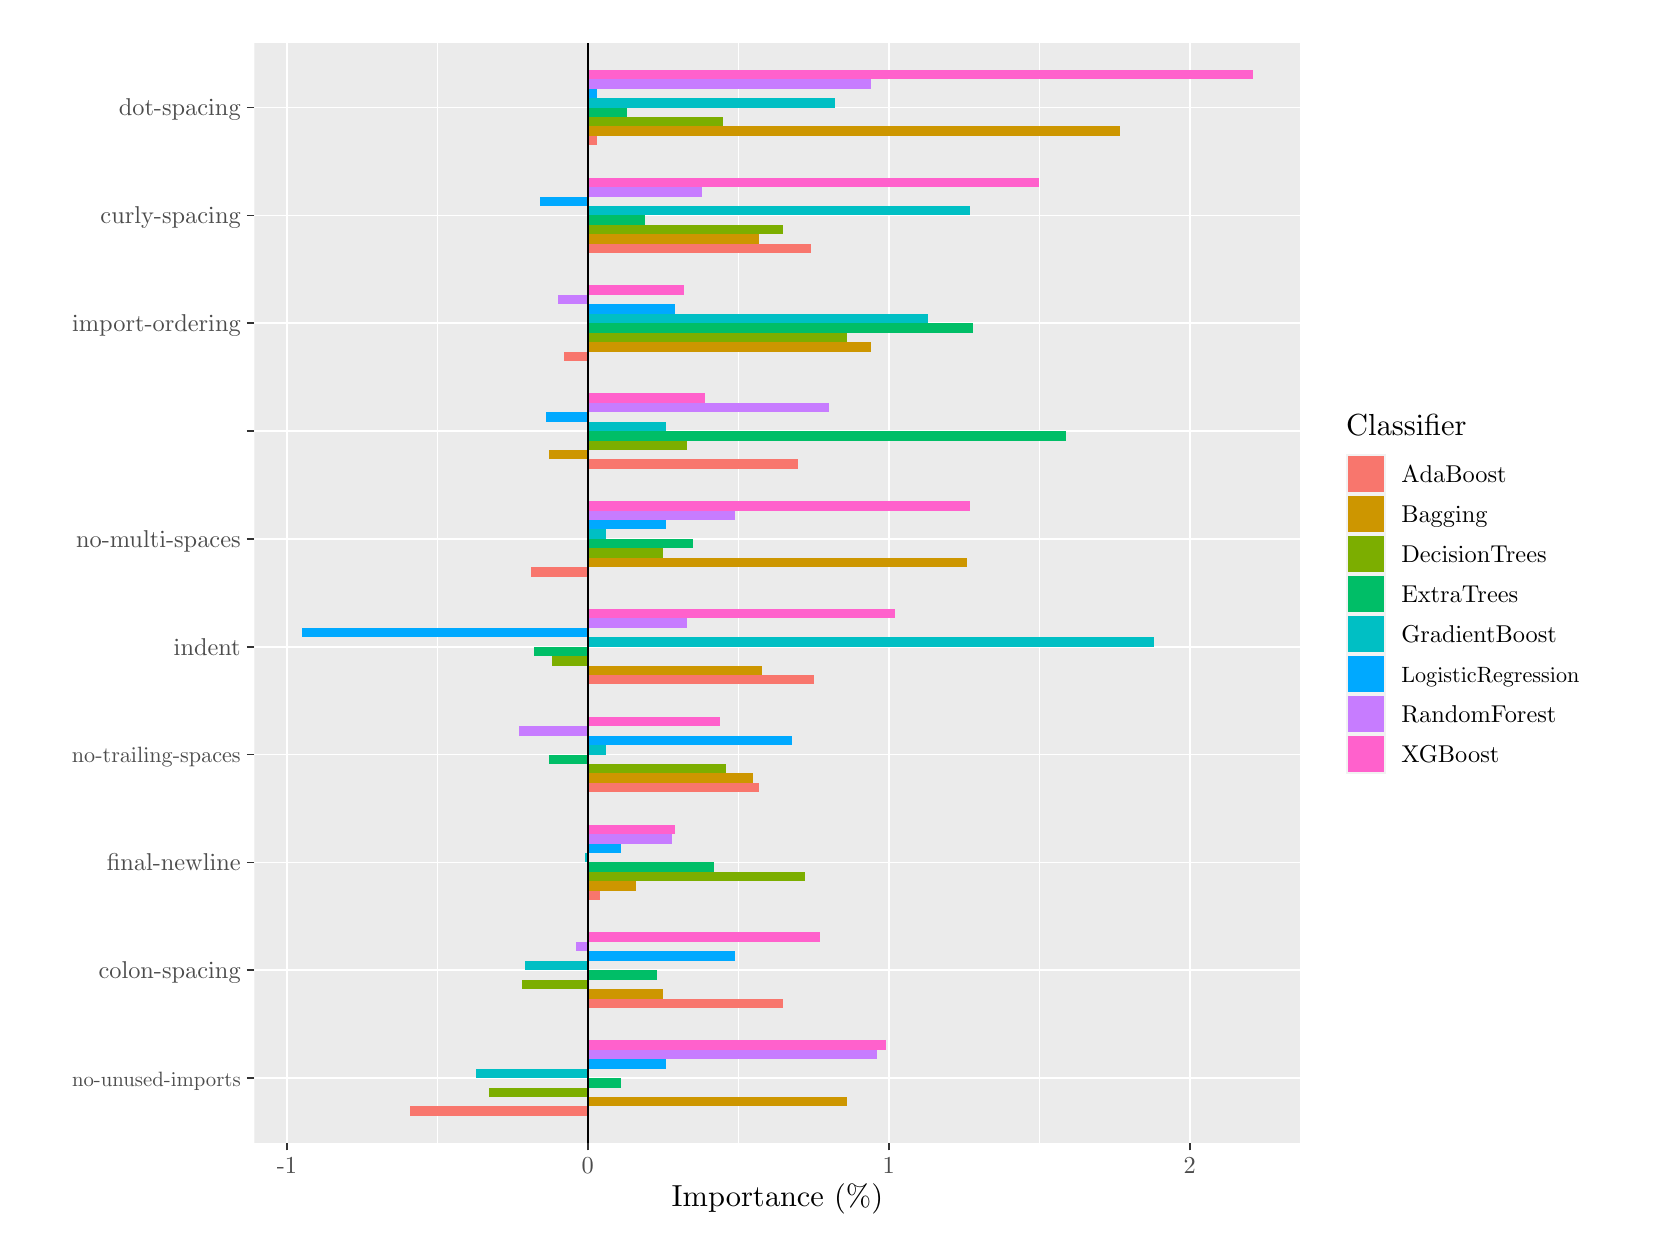
\begin{tikzpicture}[x=1pt,y=1pt]
\definecolor{fillColor}{RGB}{255,255,255}
\path[use as bounding box,fill=fillColor,fill opacity=0.00] (0,0) rectangle (578.16,433.62);
\begin{scope}
\path[clip] (  0.00,  0.00) rectangle (578.16,433.62);
\definecolor{drawColor}{RGB}{255,255,255}
\definecolor{fillColor}{RGB}{255,255,255}

\path[draw=drawColor,line width= 0.6pt,line join=round,line cap=round,fill=fillColor] (  0.00,  0.00) rectangle (578.16,433.62);
\end{scope}
\begin{scope}
\path[clip] ( 81.93, 30.69) rectangle (459.91,428.12);
\definecolor{fillColor}{gray}{0.92}

\path[fill=fillColor] ( 81.93, 30.69) rectangle (459.91,428.12);
\definecolor{drawColor}{RGB}{255,255,255}

\path[draw=drawColor,line width= 0.3pt,line join=round] (148.05, 30.69) --
	(148.05,428.12);

\path[draw=drawColor,line width= 0.3pt,line join=round] (256.78, 30.69) --
	(256.78,428.12);

\path[draw=drawColor,line width= 0.3pt,line join=round] (365.52, 30.69) --
	(365.52,428.12);

\path[draw=drawColor,line width= 0.6pt,line join=round] ( 81.93, 54.06) --
	(459.91, 54.06);

\path[draw=drawColor,line width= 0.6pt,line join=round] ( 81.93, 93.03) --
	(459.91, 93.03);

\path[draw=drawColor,line width= 0.6pt,line join=round] ( 81.93,131.99) --
	(459.91,131.99);

\path[draw=drawColor,line width= 0.6pt,line join=round] ( 81.93,170.96) --
	(459.91,170.96);

\path[draw=drawColor,line width= 0.6pt,line join=round] ( 81.93,209.92) --
	(459.91,209.92);

\path[draw=drawColor,line width= 0.6pt,line join=round] ( 81.93,248.88) --
	(459.91,248.88);

\path[draw=drawColor,line width= 0.6pt,line join=round] ( 81.93,287.85) --
	(459.91,287.85);

\path[draw=drawColor,line width= 0.6pt,line join=round] ( 81.93,326.81) --
	(459.91,326.81);

\path[draw=drawColor,line width= 0.6pt,line join=round] ( 81.93,365.78) --
	(459.91,365.78);

\path[draw=drawColor,line width= 0.6pt,line join=round] ( 81.93,404.74) --
	(459.91,404.74);

\path[draw=drawColor,line width= 0.6pt,line join=round] ( 93.68, 30.69) --
	( 93.68,428.12);

\path[draw=drawColor,line width= 0.6pt,line join=round] (202.41, 30.69) --
	(202.41,428.12);

\path[draw=drawColor,line width= 0.6pt,line join=round] (311.15, 30.69) --
	(311.15,428.12);

\path[draw=drawColor,line width= 0.6pt,line join=round] (419.89, 30.69) --
	(419.89,428.12);
\definecolor{fillColor}{RGB}{248,118,109}

\path[fill=fillColor] (202.41,391.10) rectangle (205.68,394.51);

\path[fill=fillColor] (202.41,352.14) rectangle (282.88,355.55);

\path[fill=fillColor] (193.72,313.18) rectangle (202.41,316.59);

\path[fill=fillColor] (202.41,274.21) rectangle (278.53,277.62);

\path[fill=fillColor] (181.75,235.25) rectangle (202.41,238.66);

\path[fill=fillColor] (202.41,196.28) rectangle (283.97,199.69);

\path[fill=fillColor] (202.41,157.32) rectangle (264.40,160.73);

\path[fill=fillColor] (202.41,118.36) rectangle (206.76,121.76);

\path[fill=fillColor] (202.41, 79.39) rectangle (273.09, 82.80);

\path[fill=fillColor] (138.26, 40.43) rectangle (202.41, 43.84);
\definecolor{fillColor}{RGB}{205,150,0}

\path[fill=fillColor] (202.41,394.51) rectangle (394.88,397.92);

\path[fill=fillColor] (202.41,355.55) rectangle (264.40,358.96);

\path[fill=fillColor] (202.41,316.59) rectangle (304.63,319.99);

\path[fill=fillColor] (188.28,277.62) rectangle (202.41,281.03);

\path[fill=fillColor] (202.41,238.66) rectangle (339.43,242.07);

\path[fill=fillColor] (202.41,199.69) rectangle (265.48,203.10);

\path[fill=fillColor] (202.41,160.73) rectangle (262.22,164.14);

\path[fill=fillColor] (202.41,121.76) rectangle (219.81,125.17);

\path[fill=fillColor] (202.41, 82.80) rectangle (229.60, 86.21);

\path[fill=fillColor] (202.41, 43.84) rectangle (295.93, 47.25);
\definecolor{fillColor}{RGB}{124,174,0}

\path[fill=fillColor] (202.41,397.92) rectangle (251.35,401.33);

\path[fill=fillColor] (202.41,358.96) rectangle (273.09,362.37);

\path[fill=fillColor] (202.41,319.99) rectangle (295.93,323.40);

\path[fill=fillColor] (202.41,281.03) rectangle (238.30,284.44);

\path[fill=fillColor] (202.41,242.07) rectangle (229.60,245.48);

\path[fill=fillColor] (189.37,203.10) rectangle (202.41,206.51);

\path[fill=fillColor] (202.41,164.14) rectangle (252.43,167.55);

\path[fill=fillColor] (202.41,125.17) rectangle (280.71,128.58);

\path[fill=fillColor] (178.49, 86.21) rectangle (202.41, 89.62);

\path[fill=fillColor] (166.53, 47.25) rectangle (202.41, 50.65);
\definecolor{fillColor}{RGB}{0,190,103}

\path[fill=fillColor] (202.41,401.33) rectangle (216.55,404.74);

\path[fill=fillColor] (202.41,362.37) rectangle (223.08,365.78);

\path[fill=fillColor] (202.41,323.40) rectangle (341.60,326.81);

\path[fill=fillColor] (202.41,284.44) rectangle (375.31,287.85);

\path[fill=fillColor] (202.41,245.48) rectangle (240.47,248.88);

\path[fill=fillColor] (182.84,206.51) rectangle (202.41,209.92);

\path[fill=fillColor] (188.28,167.55) rectangle (202.41,170.96);

\path[fill=fillColor] (202.41,128.58) rectangle (248.09,131.99);

\path[fill=fillColor] (202.41, 89.62) rectangle (227.42, 93.03);

\path[fill=fillColor] (202.41, 50.65) rectangle (214.38, 54.06);
\definecolor{fillColor}{RGB}{0,191,196}

\path[fill=fillColor] (202.41,404.74) rectangle (291.58,408.15);

\path[fill=fillColor] (202.41,365.78) rectangle (340.51,369.19);

\path[fill=fillColor] (202.41,326.81) rectangle (325.29,330.22);

\path[fill=fillColor] (202.41,287.85) rectangle (230.69,291.26);

\path[fill=fillColor] (202.41,248.88) rectangle (208.94,252.29);

\path[fill=fillColor] (202.41,209.92) rectangle (406.84,213.33);

\path[fill=fillColor] (202.41,170.96) rectangle (208.94,174.37);

\path[fill=fillColor] (201.33,131.99) rectangle (202.41,135.40);

\path[fill=fillColor] (179.58, 93.03) rectangle (202.41, 96.44);

\path[fill=fillColor] (162.18, 54.06) rectangle (202.41, 57.47);
\definecolor{fillColor}{RGB}{0,169,255}

\path[fill=fillColor] (202.41,408.15) rectangle (205.68,411.56);

\path[fill=fillColor] (185.02,369.19) rectangle (202.41,372.60);

\path[fill=fillColor] (202.41,330.22) rectangle (233.95,333.63);

\path[fill=fillColor] (187.19,291.26) rectangle (202.41,294.67);

\path[fill=fillColor] (202.41,252.29) rectangle (230.69,255.70);

\path[fill=fillColor] ( 99.11,213.33) rectangle (202.41,216.74);

\path[fill=fillColor] (202.41,174.37) rectangle (276.36,177.78);

\path[fill=fillColor] (202.41,135.40) rectangle (214.38,138.81);

\path[fill=fillColor] (202.41, 96.44) rectangle (255.70, 99.85);

\path[fill=fillColor] (202.41, 57.47) rectangle (230.69, 60.88);
\definecolor{fillColor}{RGB}{199,124,255}

\path[fill=fillColor] (202.41,411.56) rectangle (304.63,414.97);

\path[fill=fillColor] (202.41,372.60) rectangle (243.74,376.01);

\path[fill=fillColor] (191.54,333.63) rectangle (202.41,337.04);

\path[fill=fillColor] (202.41,294.67) rectangle (289.41,298.08);

\path[fill=fillColor] (202.41,255.70) rectangle (255.70,259.11);

\path[fill=fillColor] (202.41,216.74) rectangle (238.30,220.15);

\path[fill=fillColor] (177.41,177.78) rectangle (202.41,181.18);

\path[fill=fillColor] (202.41,138.81) rectangle (232.86,142.22);

\path[fill=fillColor] (198.07, 99.85) rectangle (202.41,103.26);

\path[fill=fillColor] (202.41, 60.88) rectangle (306.80, 64.29);
\definecolor{fillColor}{RGB}{255,97,204}

\path[fill=fillColor] (202.41,414.97) rectangle (442.73,418.38);

\path[fill=fillColor] (202.41,376.01) rectangle (365.52,379.41);

\path[fill=fillColor] (202.41,337.04) rectangle (237.21,340.45);

\path[fill=fillColor] (202.41,298.08) rectangle (244.82,301.49);

\path[fill=fillColor] (202.41,259.11) rectangle (340.51,262.52);

\path[fill=fillColor] (202.41,220.15) rectangle (313.33,223.56);

\path[fill=fillColor] (202.41,181.18) rectangle (250.26,184.59);

\path[fill=fillColor] (202.41,142.22) rectangle (233.95,145.63);

\path[fill=fillColor] (202.41,103.26) rectangle (286.14,106.67);

\path[fill=fillColor] (202.41, 64.29) rectangle (310.07, 67.70);
\definecolor{drawColor}{RGB}{0,0,0}

\path[draw=drawColor,line width= 0.6pt,line join=round] (202.41, 30.69) -- (202.41,428.12);
\end{scope}
\begin{scope}
\path[clip] (  0.00,  0.00) rectangle (578.16,433.62);
\definecolor{drawColor}{gray}{0.30}

\node[text=drawColor,anchor=base east,inner sep=0pt, outer sep=0pt, scale=  0.75] at ( 76.98, 51.03) {no-unused-imports};

\node[text=drawColor,anchor=base east,inner sep=0pt, outer sep=0pt, scale=  0.88] at ( 76.98, 90.00) {colon-spacing};

\node[text=drawColor,anchor=base east,inner sep=0pt, outer sep=0pt, scale=  0.88] at ( 76.98,128.96) {final-newline};

\node[text=drawColor,anchor=base east,inner sep=0pt, outer sep=0pt, scale=  0.80] at ( 76.98,167.93) {no-trailing-spaces};

\node[text=drawColor,anchor=base east,inner sep=0pt, outer sep=0pt, scale=  0.88] at ( 76.98,206.89) {indent};

\node[text=drawColor,anchor=base east,inner sep=0pt, outer sep=0pt, scale=  0.88] at ( 76.98,245.85) {no-multi-spaces};

\node[text=drawColor,anchor=base east,inner sep=0pt, outer sep=0pt, scale=  0.88] at ( 76.98,323.78) {import-ordering};

\node[text=drawColor,anchor=base east,inner sep=0pt, outer sep=0pt, scale=  0.88] at ( 76.98,362.75) {curly-spacing};

\node[text=drawColor,anchor=base east,inner sep=0pt, outer sep=0pt, scale=  0.88] at ( 76.98,401.71) {dot-spacing};
\end{scope}
\begin{scope}
\path[clip] (  0.00,  0.00) rectangle (578.16,433.62);
\definecolor{drawColor}{gray}{0.20}

\path[draw=drawColor,line width= 0.6pt,line join=round] ( 79.18, 54.06) --
	( 81.93, 54.06);

\path[draw=drawColor,line width= 0.6pt,line join=round] ( 79.18, 93.03) --
	( 81.93, 93.03);

\path[draw=drawColor,line width= 0.6pt,line join=round] ( 79.18,131.99) --
	( 81.93,131.99);

\path[draw=drawColor,line width= 0.6pt,line join=round] ( 79.18,170.96) --
	( 81.93,170.96);

\path[draw=drawColor,line width= 0.6pt,line join=round] ( 79.18,209.92) --
	( 81.93,209.92);

\path[draw=drawColor,line width= 0.6pt,line join=round] ( 79.18,248.88) --
	( 81.93,248.88);

\path[draw=drawColor,line width= 0.6pt,line join=round] ( 79.18,287.85) --
	( 81.93,287.85);

\path[draw=drawColor,line width= 0.6pt,line join=round] ( 79.18,326.81) --
	( 81.93,326.81);

\path[draw=drawColor,line width= 0.6pt,line join=round] ( 79.18,365.78) --
	( 81.93,365.78);

\path[draw=drawColor,line width= 0.6pt,line join=round] ( 79.18,404.74) --
	( 81.93,404.74);
\end{scope}
\begin{scope}
\path[clip] (  0.00,  0.00) rectangle (578.16,433.62);
\definecolor{drawColor}{gray}{0.20}

\path[draw=drawColor,line width= 0.6pt,line join=round] ( 93.68, 27.94) --
	( 93.68, 30.69);

\path[draw=drawColor,line width= 0.6pt,line join=round] (202.41, 27.94) --
	(202.41, 30.69);

\path[draw=drawColor,line width= 0.6pt,line join=round] (311.15, 27.94) --
	(311.15, 30.69);

\path[draw=drawColor,line width= 0.6pt,line join=round] (419.89, 27.94) --
	(419.89, 30.69);
\end{scope}
\begin{scope}
\path[clip] (  0.00,  0.00) rectangle (578.16,433.62);
\definecolor{drawColor}{gray}{0.30}

\node[text=drawColor,anchor=base,inner sep=0pt, outer sep=0pt, scale=  0.88] at ( 93.68, 19.68) {-1};

\node[text=drawColor,anchor=base,inner sep=0pt, outer sep=0pt, scale=  0.88] at (202.41, 19.68) {0};

\node[text=drawColor,anchor=base,inner sep=0pt, outer sep=0pt, scale=  0.88] at (311.15, 19.68) {1};

\node[text=drawColor,anchor=base,inner sep=0pt, outer sep=0pt, scale=  0.88] at (419.89, 19.68) {2};
\end{scope}
\begin{scope}
\path[clip] (  0.00,  0.00) rectangle (578.16,433.62);
\definecolor{drawColor}{RGB}{0,0,0}

\node[text=drawColor,anchor=base,inner sep=0pt, outer sep=0pt, scale=  1.10] at (270.92,  7.64) {Importance (\%)};
\end{scope}
\begin{scope}
\path[clip] (  0.00,  0.00) rectangle (578.16,433.62);
\definecolor{fillColor}{RGB}{255,255,255}

\path[fill=fillColor] (470.91,158.48) rectangle (572.66,300.33);
\end{scope}
\begin{scope}
\path[clip] (  0.00,  0.00) rectangle (578.16,433.62);
\definecolor{drawColor}{RGB}{0,0,0}

\node[text=drawColor,anchor=base west,inner sep=0pt, outer sep=0pt, scale=  1.10] at (476.41,286.18) {Classifier};
\end{scope}
\begin{scope}
\path[clip] (  0.00,  0.00) rectangle (578.16,433.62);
\definecolor{fillColor}{gray}{0.95}

\path[fill=fillColor] (476.41,265.16) rectangle (490.86,279.61);
\end{scope}
\begin{scope}
\path[clip] (  0.00,  0.00) rectangle (578.16,433.62);
\definecolor{fillColor}{RGB}{248,118,109}

\path[fill=fillColor] (477.12,265.87) rectangle (490.15,278.90);
\end{scope}
\begin{scope}
\path[clip] (  0.00,  0.00) rectangle (578.16,433.62);
\definecolor{fillColor}{gray}{0.95}

\path[fill=fillColor] (476.41,250.70) rectangle (490.86,265.16);
\end{scope}
\begin{scope}
\path[clip] (  0.00,  0.00) rectangle (578.16,433.62);
\definecolor{fillColor}{RGB}{205,150,0}

\path[fill=fillColor] (477.12,251.42) rectangle (490.15,264.45);
\end{scope}
\begin{scope}
\path[clip] (  0.00,  0.00) rectangle (578.16,433.62);
\definecolor{fillColor}{gray}{0.95}

\path[fill=fillColor] (476.41,236.25) rectangle (490.86,250.70);
\end{scope}
\begin{scope}
\path[clip] (  0.00,  0.00) rectangle (578.16,433.62);
\definecolor{fillColor}{RGB}{124,174,0}

\path[fill=fillColor] (477.12,236.96) rectangle (490.15,249.99);
\end{scope}
\begin{scope}
\path[clip] (  0.00,  0.00) rectangle (578.16,433.62);
\definecolor{fillColor}{gray}{0.95}

\path[fill=fillColor] (476.41,221.80) rectangle (490.86,236.25);
\end{scope}
\begin{scope}
\path[clip] (  0.00,  0.00) rectangle (578.16,433.62);
\definecolor{fillColor}{RGB}{0,190,103}

\path[fill=fillColor] (477.12,222.51) rectangle (490.15,235.54);
\end{scope}
\begin{scope}
\path[clip] (  0.00,  0.00) rectangle (578.16,433.62);
\definecolor{fillColor}{gray}{0.95}

\path[fill=fillColor] (476.41,207.34) rectangle (490.86,221.80);
\end{scope}
\begin{scope}
\path[clip] (  0.00,  0.00) rectangle (578.16,433.62);
\definecolor{fillColor}{RGB}{0,191,196}

\path[fill=fillColor] (477.12,208.05) rectangle (490.15,221.08);
\end{scope}
\begin{scope}
\path[clip] (  0.00,  0.00) rectangle (578.16,433.62);
\definecolor{fillColor}{gray}{0.95}

\path[fill=fillColor] (476.41,192.89) rectangle (490.86,207.34);
\end{scope}
\begin{scope}
\path[clip] (  0.00,  0.00) rectangle (578.16,433.62);
\definecolor{fillColor}{RGB}{0,169,255}

\path[fill=fillColor] (477.12,193.60) rectangle (490.15,206.63);
\end{scope}
\begin{scope}
\path[clip] (  0.00,  0.00) rectangle (578.16,433.62);
\definecolor{fillColor}{gray}{0.95}

\path[fill=fillColor] (476.41,178.43) rectangle (490.86,192.89);
\end{scope}
\begin{scope}
\path[clip] (  0.00,  0.00) rectangle (578.16,433.62);
\definecolor{fillColor}{RGB}{199,124,255}

\path[fill=fillColor] (477.12,179.15) rectangle (490.15,192.18);
\end{scope}
\begin{scope}
\path[clip] (  0.00,  0.00) rectangle (578.16,433.62);
\definecolor{fillColor}{gray}{0.95}

\path[fill=fillColor] (476.41,163.98) rectangle (490.86,178.43);
\end{scope}
\begin{scope}
\path[clip] (  0.00,  0.00) rectangle (578.16,433.62);
\definecolor{fillColor}{RGB}{255,97,204}

\path[fill=fillColor] (477.12,164.69) rectangle (490.15,177.72);
\end{scope}
\begin{scope}
\path[clip] (  0.00,  0.00) rectangle (578.16,433.62);
\definecolor{drawColor}{RGB}{0,0,0}

\node[text=drawColor,anchor=base west,inner sep=0pt, outer sep=0pt, scale=  0.88] at (496.36,269.35) {AdaBoost};
\end{scope}
\begin{scope}
\path[clip] (  0.00,  0.00) rectangle (578.16,433.62);
\definecolor{drawColor}{RGB}{0,0,0}

\node[text=drawColor,anchor=base west,inner sep=0pt, outer sep=0pt, scale=  0.88] at (496.36,254.90) {Bagging};
\end{scope}
\begin{scope}
\path[clip] (  0.00,  0.00) rectangle (578.16,433.62);
\definecolor{drawColor}{RGB}{0,0,0}

\node[text=drawColor,anchor=base west,inner sep=0pt, outer sep=0pt, scale=  0.88] at (496.36,240.45) {DecisionTrees};
\end{scope}
\begin{scope}
\path[clip] (  0.00,  0.00) rectangle (578.16,433.62);
\definecolor{drawColor}{RGB}{0,0,0}

\node[text=drawColor,anchor=base west,inner sep=0pt, outer sep=0pt, scale=  0.88] at (496.36,225.99) {ExtraTrees};
\end{scope}
\begin{scope}
\path[clip] (  0.00,  0.00) rectangle (578.16,433.62);
\definecolor{drawColor}{RGB}{0,0,0}

\node[text=drawColor,anchor=base west,inner sep=0pt, outer sep=0pt, scale=  0.88] at (496.36,211.54) {GradientBoost};
\end{scope}
\begin{scope}
\path[clip] (  0.00,  0.00) rectangle (578.16,433.62);
\definecolor{drawColor}{RGB}{0,0,0}

\node[text=drawColor,anchor=base west,inner sep=0pt, outer sep=0pt, scale=  0.80] at (496.36,197.08) {LogisticRegression};
\end{scope}
\begin{scope}
\path[clip] (  0.00,  0.00) rectangle (578.16,433.62);
\definecolor{drawColor}{RGB}{0,0,0}

\node[text=drawColor,anchor=base west,inner sep=0pt, outer sep=0pt, scale=  0.88] at (496.36,182.63) {RandomForest};
\end{scope}
\begin{scope}
\path[clip] (  0.00,  0.00) rectangle (578.16,433.62);
\definecolor{drawColor}{RGB}{0,0,0}

\node[text=drawColor,anchor=base west,inner sep=0pt, outer sep=0pt, scale=  0.88] at (496.36,168.18) {XGBoost};
\end{scope}
\end{tikzpicture}
